\chapter{Stato dell'arte}
\label{statodellarte}

\newpage
\section{Machine Learning}

\newpage
\section{Reti neurali}

\subsection{Percettrone Multistrato}
\subsection{Adversarial Networks}
The adversarial modeling framework is most straightforward to apply when the models are both multilayer perceptrons. To learn the generator's distribution $p_g$ over data $\bm{x}$, we
define a prior on input noise variables $p_{\bm{z}}(\bm{z})$, then represent a
mapping to data space as $G(\bm{z}; \theta_g)$, where $G$ is a differentiable function
represented by a multilayer perceptron with parameters $\theta_g$. We also define a second
multilayer perceptron $D(\bm{x}; \theta_d)$ that outputs a single scalar. $D(\bm{x})$ represents
the probability that $\bm{x}$ came from the data rather than $p_g$. We train $D$ to maximize the
probability of assigning the correct label to both training examples and samples from $G$.
We simultaneously train $G$ to minimize $\log(1-D(G(\bm{z})))$:

In other words, $D$ and $G$ play the following two-player minimax game with value function $V(G, D)$: 

\begin{equation}
\label{eq:minimaxgame-definition}
\min_G \max_D V(D, G) = \mathbb{E}_{\bm{x} \sim p_{\text{data}}(\bm{x})}[\log D(\bm{x})] + \mathbb{E}_{\bm{z} \sim p_{\bm{z}}(\bm{z})}[\log (1 - D(G(\bm{z})))].
\end{equation}

In the next section, we present a theoretical analysis of adversarial nets,
essentially showing that the training criterion allows one to recover the data
generating distribution as $G$ and $D$ are given enough capacity, i.e., in the
non-parametric limit. See Figure~\ref{fig:intuition} for a less formal, more pedagogical
explanation of the approach.
In practice, we must implement the game using an iterative, numerical approach. Optimizing $D$ to completion in the
inner loop of training is computationally prohibitive,
and on finite datasets would result in overfitting. Instead, we alternate between $k$ steps
of optimizing $D$ and one step of optimizing $G$. This results in $D$ being maintained
near its optimal solution, so long as $G$ changes slowly enough. This strategy is analogous
to the way that SML/PCD~\citep{Younes1999,Tieleman08} training maintains samples from a Markov chain from one
learning step to the next in order to avoid burning in a Markov chain as part of the inner loop
of learning. The procedure is formally presented
in Algorithm~\ref{alg:AGF}.

In practice, equation~\ref{eq:minimaxgame-definition} may not provide sufficient gradient for $G$ to learn
well. Early in learning, when $G$ is poor, $D$ can reject samples with high confidence because they are
clearly different from the training data. In this case, $\log ( 1- D(G(\bm{z})))$ saturates. Rather than
training $G$ to minimize $\log (1 - D(G(\bm{z})))$ we can train $G$ to maximize $\log D(G(\bm{z}))$.
This objective function results in the same fixed point of the dynamics of $G$ and $D$ but provides much
stronger gradients early in learning.


%explains the intuition
%behind these asymptotic consistency results. When $D$ tracks its optimum,
%it classifies $x$'s according to Bayes rule, i.e., 
%$D^*(x) = \frac{P_X}{P_X(x) + P_G(x)}$, and the gradient of $D(G(z))$ on $G(z)$ pushes
%probability mass in the direction of increasing value of $D$, i.e., towards regions 
%where $P_X(x)>P_G(x)$. This necessarily pulls probability mass away from
%regions where $P_X(x)<P_G(x)$. This happens because on the border of regions
%where $P_X(x)>P_G(x)$ the derivative of $D^*$ must point inside, and vice-versa.
%Hence the gradient pushes $G$ towards allocating more mass where it did not put enough,
%and vice-versa. A more formal proof of convergence is presented in Section~\ref{},
%also showing that the criterion is consistent, so long as $D$ is allowed to track
%its optimum, i.e., $G$ is making small changes between optimizations of $D$.

\begin{figure}[h]
\begin{tabular}{m{3cm}m{3cm}m{3cm}m{0.1cm}m{3cm}}
    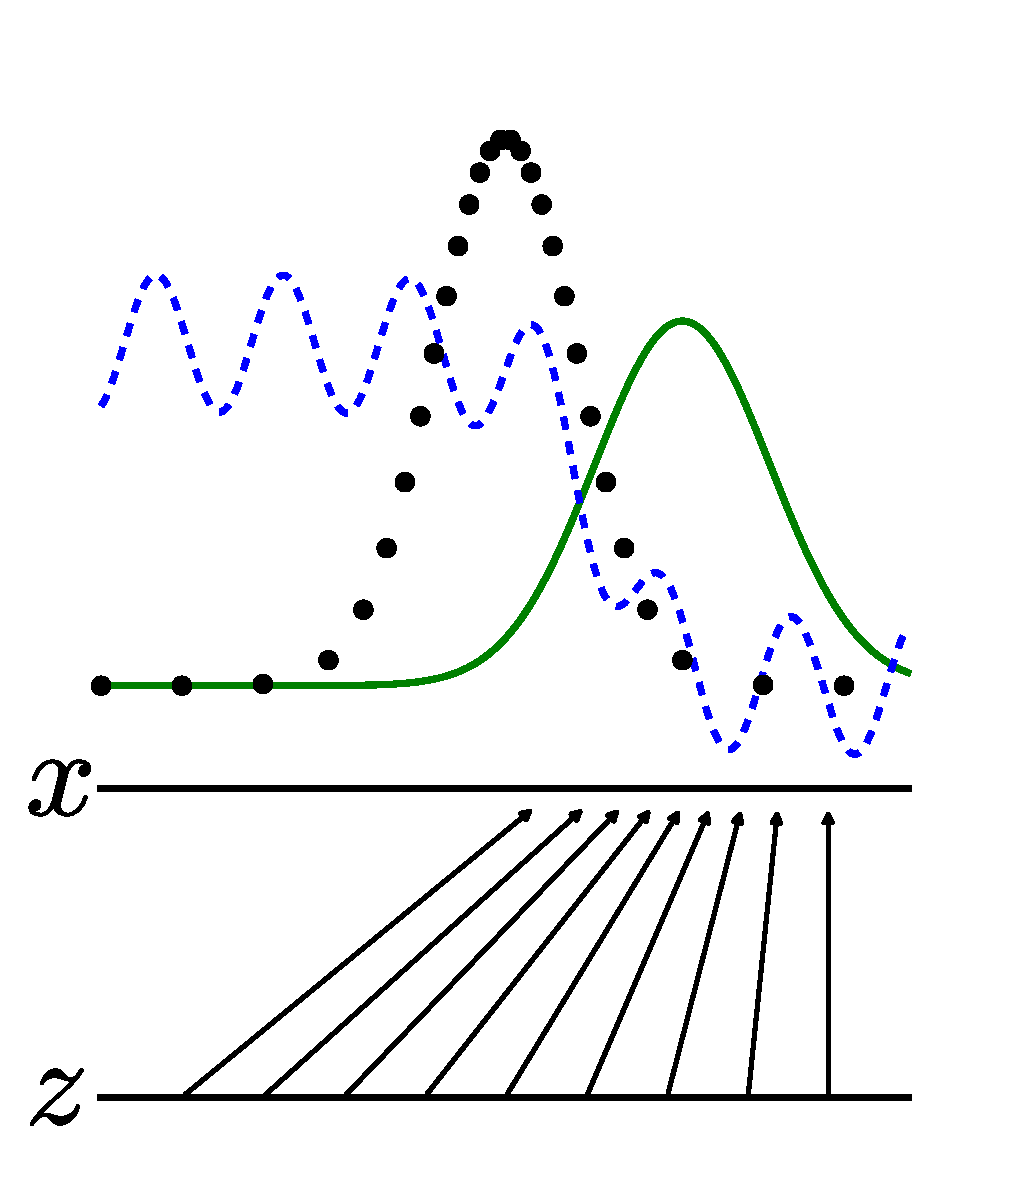
\includegraphics[width=3cm, height=4cm]{fig1.pdf} 
    &  
    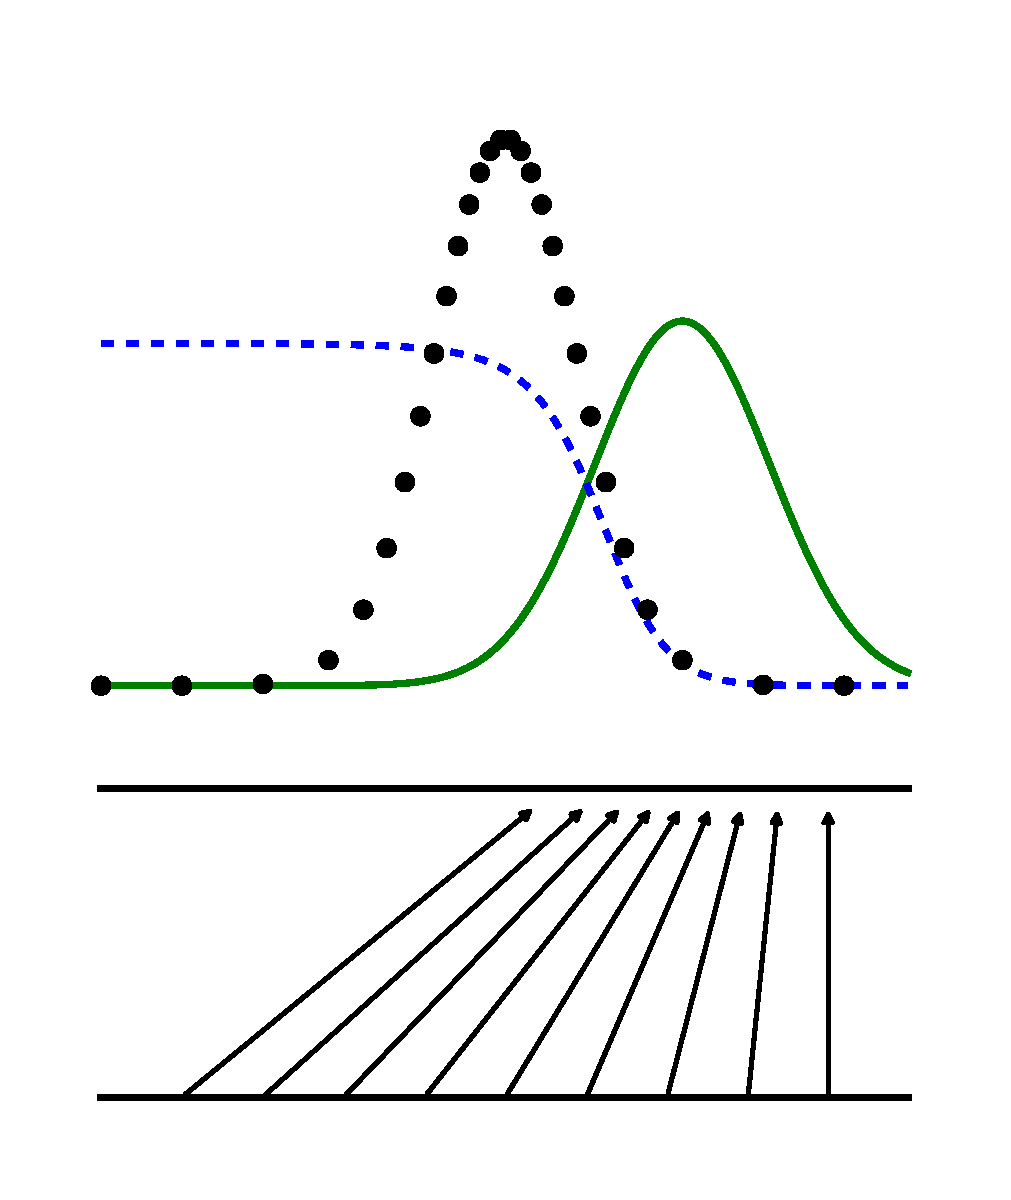
\includegraphics[width=3cm, height=4cm]{fig2.pdf}
    & 
    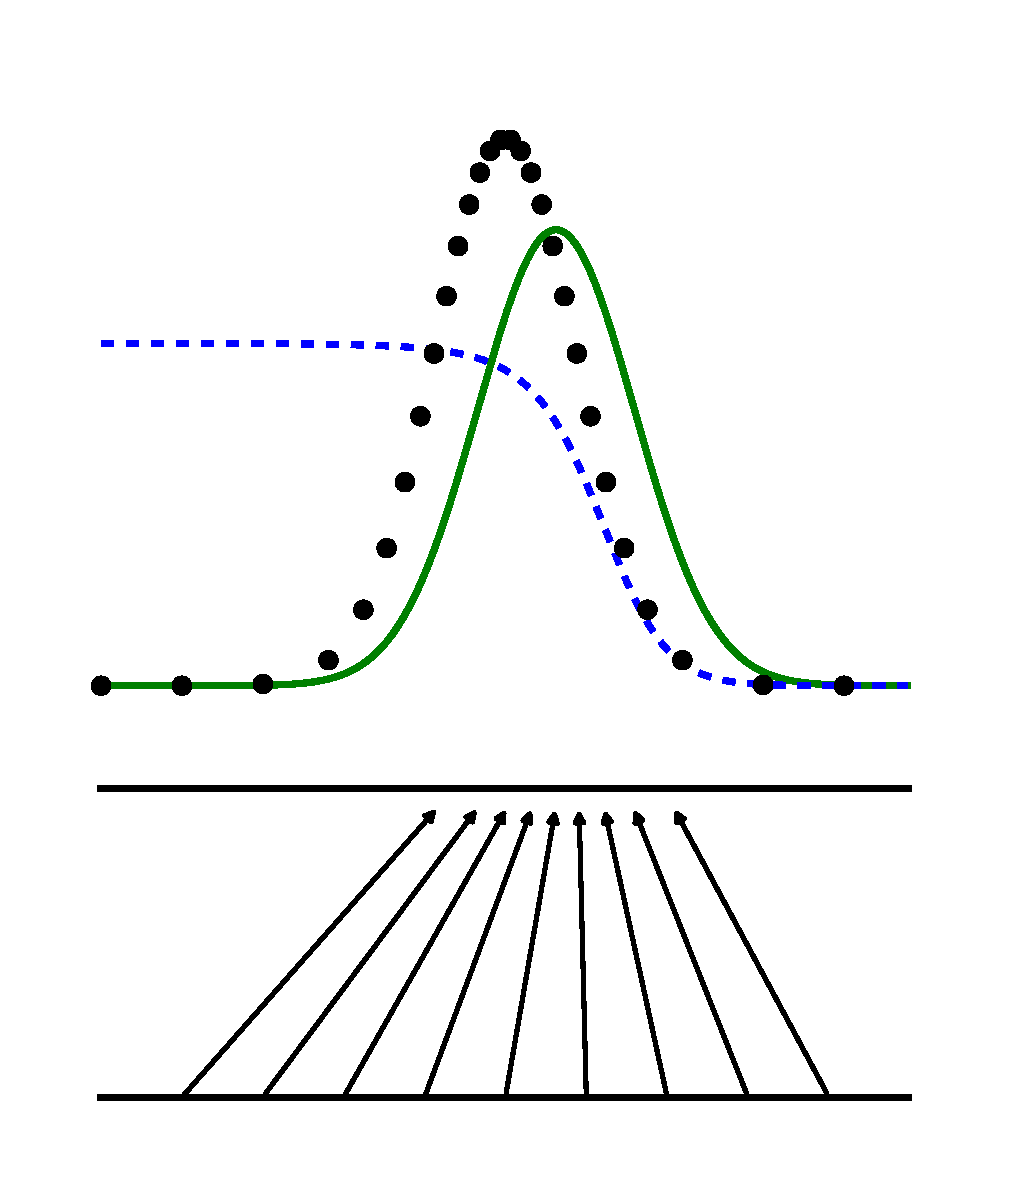
\includegraphics[width=3cm, height=4cm]{fig3.pdf}
    &
    \dots
    &
    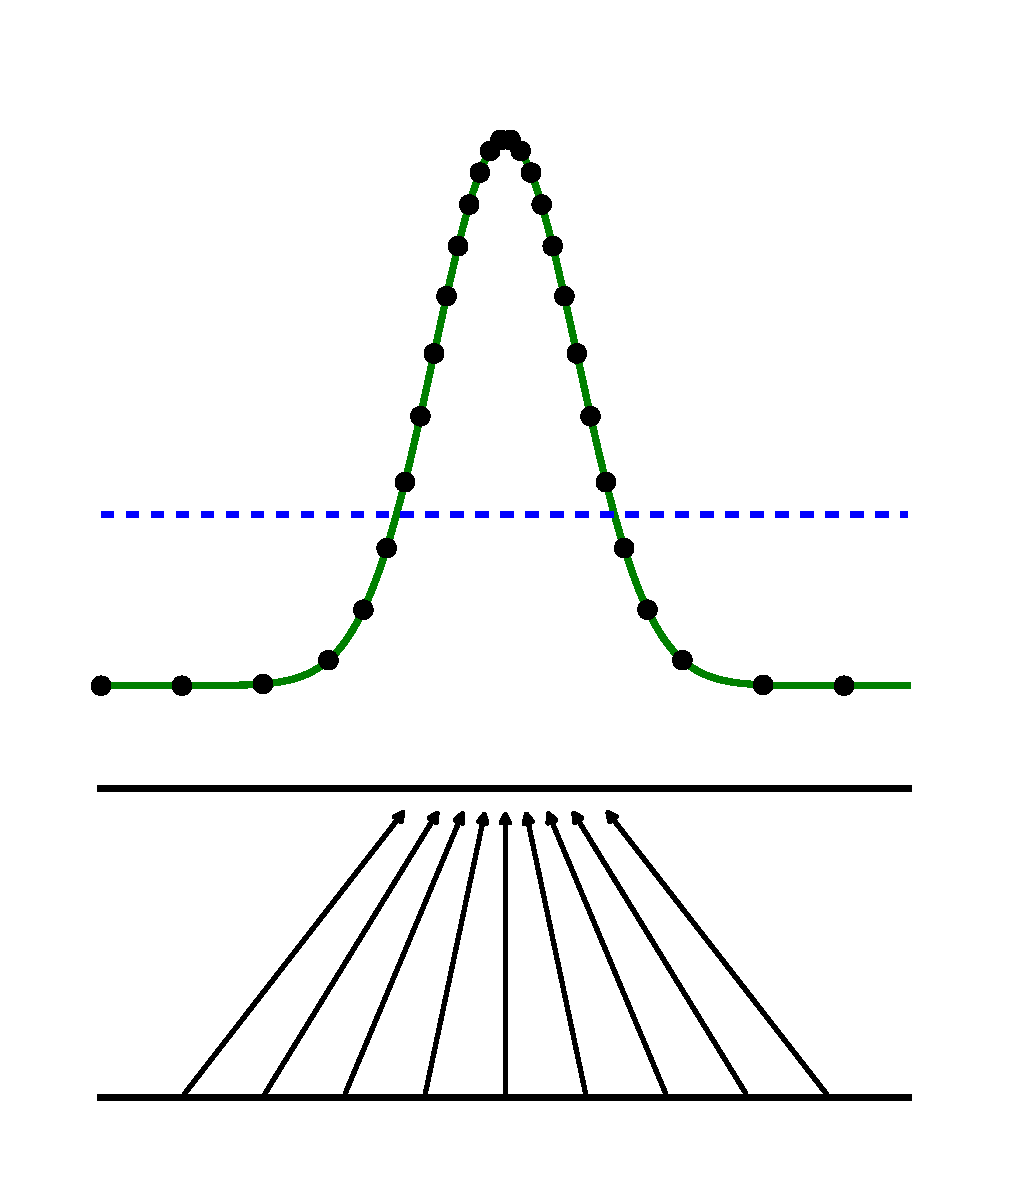
\includegraphics[width=3cm, height=4cm]{fig4.pdf}
    \\
    \centering (a)
    & 
    \centering (b) 
    & 
    \centering (c) 
    &  
    & 
    \centering (d)
\end{tabular}

\caption{\small
Generative adversarial nets are trained by simultaneously updating the \textbf{d}iscriminative 
distribution ($D$, blue, dashed line) so that it discriminates between samples from
the data generating distribution (black, dotted line)
$p_{\bm{x}}$ 
from those of the \textbf{g}enerative distribution $p_g$ (G) (green, solid line).
The lower horizontal line is the domain from which $\bm{z}$ is sampled, in this case uniformly.
The horizontal line above is part of the domain of $\bm{x}$. The upward arrows show
how the mapping $\bm{x}=G(\bm{z})$ imposes the non-uniform distribution $p_g$ on transformed samples.
$G$ contracts in regions of high density and expands in regions of low density of $p_g$.
(a) Consider an adversarial pair near convergence: $p_g$ is similar to $p_\text{data}$ and
$D$ is a partially accurate classifier.
(b) In the inner loop of the algorithm $D$ is trained to discriminate samples from data,
converging to
$D^*(\bm{x}) = 
\frac{
    p_\text{data}(\bm{x})
    }{
        p_\text{data}(\bm{x}) + p_g(\bm{x})}
$. 
(c) After an update to $G$, gradient of $D$ has guided $G(\bm{z})$ to flow to regions that are more likely
to be classified as data.
(d) After several steps of training, if $G$ and $D$ have enough capacity, they will reach a point at which
both cannot improve because $p_g = p_\text{data}$.
The discriminator is unable to differentiate between the two 
distributions, i.e. $D(\bm{x}) = \frac{1}{2}$.
}
\label{fig:intuition}
\end{figure}



\begin{algorithm}[ht]
\caption{\small Minibatch stochastic gradient descent training of generative adversarial nets.
The number of steps to apply to the discriminator, $k$, is a hyperparameter. We used $k=1$, the
least expensive option, in our experiments.
}
\begin{algorithmic}
\label{alg:AGF}
\FOR{number of training iterations}
  \FOR{$k$ steps}
    \STATE{$\bullet$ Sample minibatch of $m$ noise samples $\{ \bm{z}^{(1)}, \dots, \bm{z}^{(m)} \}$ from noise prior $p_g(\bm{z})$.}
    \STATE{$\bullet$ Sample minibatch of $m$ examples $\{ \bm{x}^{(1)}, \dots, \bm{x}^{(m)} \}$ from data generating distribution $p_\text{data}(\bm{x})$.}
    \STATE{$\bullet$ Update the discriminator by ascending its stochastic gradient:
        \[
            \nabla_{\theta_d} \frac{1}{m} \sum_{i=1}^m \left[
            \log D\left(\bm{x}^{(i)}\right)
            + \log \left(1-D\left(G\left(\bm{z}^{(i)}\right)\right)\right)
            \right].
        \]}
    %parameters $\theta_d$ of discriminator $D$
   %in the direction of the stochastic gradient of the binomial cross-entropy
   %for $D$ predicting whether its argument comes from $p_\text{data}(\bm{x})$ (target = 1, input = $\bm{x}$) or
   %$P_g$ (target = 0, input = $G(\bm{z})$), i.e., towards minimizing
   % \mbox{$-\log D(\bm{x}) - \log(1 - D(G(\bm{z})))$}.}
   \ENDFOR
  \STATE{$\bullet$ Sample minibatch of $m$ noise samples $\{ \bm{z}^{(1)}, \dots, \bm{z}^{(m)} \}$ from noise prior $p_g(\bm{z})$.}
    \STATE{$\bullet$ Update the generator by descending its stochastic gradient:
        \[
            \nabla_{\theta_g} \frac{1}{m} \sum_{i=1}^m
            \log \left(1-D\left(G\left(\bm{z}^{(i)}\right)\right)\right)
            .
        \]}
  \ENDFOR
  \\The gradient-based updates can use any standard gradient-based learning rule. We used momentum in our experiments.
\end{algorithmic}
\end{algorithm}

\subsubsection{Autoencoder}

\newpage
\section{Adversarial Learning}
??? come?
